\begin{figure} [h!]
\begin{center}
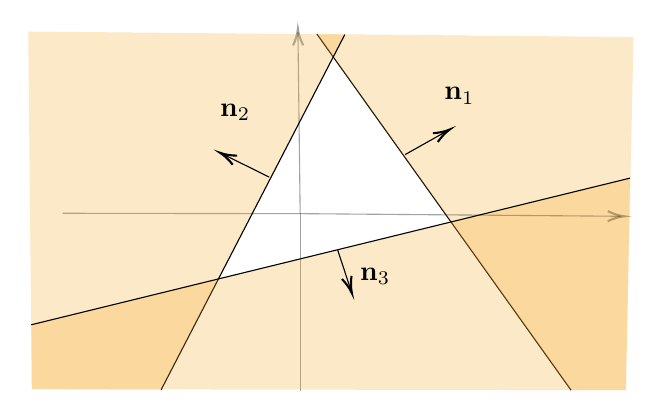
\begin{tikzpicture}[x=0.55pt,y=0.55pt,yscale=-1,xscale=1]
%uncomment if require: \path (0,300); %set diagram left start at 0, and has height of 300

%Straight Lines [id:da6725207022045878] 
\draw    (335,25.5) -- (502,259.5) ;
%Shape: Polygon [id:ds5954714579613014] 
\draw  [draw opacity=0][fill={rgb, 255:red, 245; green, 166; blue, 35 }  ,fill opacity=0.25 ] (543,27.5) -- (538,259.5) -- (502,259.5) -- (335,25.5) -- cycle ;
%Straight Lines [id:da6659527637106164] 
\draw    (393,104.67) -- (420.59,89.15) ;
\draw [shift={(422.33,88.17)}, rotate = 510.64] [color={rgb, 255:red, 0; green, 0; blue, 0 }  ][line width=0.75]    (10.93,-3.29) .. controls (6.95,-1.4) and (3.31,-0.3) .. (0,0) .. controls (3.31,0.3) and (6.95,1.4) .. (10.93,3.29)   ;
%Straight Lines [id:da7520623163425082] 
\draw [color={rgb, 255:red, 0; green, 0; blue, 0 }  ,draw opacity=0.36 ]   (324,143.5) -- (322.52,24) ;
\draw [shift={(322.5,22)}, rotate = 449.29] [color={rgb, 255:red, 0; green, 0; blue, 0 }  ,draw opacity=0.36 ][line width=0.75]    (10.93,-3.29) .. controls (6.95,-1.4) and (3.31,-0.3) .. (0,0) .. controls (3.31,0.3) and (6.95,1.4) .. (10.93,3.29)   ;
%Straight Lines [id:da8019604271716267] 
\draw [color={rgb, 255:red, 0; green, 0; blue, 0 }  ,draw opacity=0.36 ]   (324,143.5) -- (324,260.25) ;
%Straight Lines [id:da9975734887022978] 
\draw [color={rgb, 255:red, 0; green, 0; blue, 0 }  ,draw opacity=0.36 ]   (168,143.25) -- (324,143.5) ;
%Straight Lines [id:da6037170480132432] 
\draw [color={rgb, 255:red, 0; green, 0; blue, 0 }  ,draw opacity=0.36 ]   (324,143.5) -- (535,145.23) ;
\draw [shift={(537,145.25)}, rotate = 180.47] [color={rgb, 255:red, 0; green, 0; blue, 0 }  ,draw opacity=0.36 ][line width=0.75]    (10.93,-3.29) .. controls (6.95,-1.4) and (3.31,-0.3) .. (0,0) .. controls (3.31,0.3) and (6.95,1.4) .. (10.93,3.29)   ;
%Shape: Polygon [id:ds2697615572268972] 
\draw  [draw opacity=0][fill={rgb, 255:red, 245; green, 166; blue, 35 }  ,fill opacity=0.25 ] (353.33,25.83) -- (232.67,259.17) -- (147.67,258.83) -- (145.33,23.83) -- cycle ;
%Straight Lines [id:da5531097421453206] 
\draw    (353.33,25.83) -- (232.67,259.17) ;
%Shape: Polygon [id:ds45225811581456] 
\draw  [draw opacity=0][fill={rgb, 255:red, 245; green, 166; blue, 35 }  ,fill opacity=0.25 ] (540.67,120.17) -- (538,259.5) -- (147.67,258.83) -- (147.33,216.5) -- cycle ;
%Straight Lines [id:da2591402586511129] 
\draw    (540.67,120.17) -- (147.33,216.5) ;
%Straight Lines [id:da6357606107432212] 
\draw    (303.67,119.5) -- (273.13,104.39) ;
\draw [shift={(271.33,103.5)}, rotate = 386.33000000000004] [color={rgb, 255:red, 0; green, 0; blue, 0 }  ][line width=0.75]    (10.93,-3.29) .. controls (6.95,-1.4) and (3.31,-0.3) .. (0,0) .. controls (3.31,0.3) and (6.95,1.4) .. (10.93,3.29)   ;
%Straight Lines [id:da663892331852407] 
\draw    (348.67,167.5) -- (357.37,193.93) ;
\draw [shift={(358,195.83)}, rotate = 251.76999999999998] [color={rgb, 255:red, 0; green, 0; blue, 0 }  ][line width=0.75]    (10.93,-3.29) .. controls (6.95,-1.4) and (3.31,-0.3) .. (0,0) .. controls (3.31,0.3) and (6.95,1.4) .. (10.93,3.29)   ;

% Text Node
\draw (417,59) node [anchor=north west][inner sep=0.75pt]    {$\mathbf n_{1}$};
% Text Node
\draw (269.67,70) node [anchor=north west][inner sep=0.75pt]    {$\mathbf n_{2}$};
% Text Node
\draw (361.67,177.67) node [anchor=north west][inner sep=0.75pt]    {$\mathbf n_{3}$};

\end{tikzpicture}

\end{center} 
% \caption{Visualization of trajectory generation done in the developed software}
\end{figure}